\chapter{Method}
\label{chapter:method}
\epigraph{\textit{Du bist schön, aber dafür kannst du nichts.
Weder Lesen, noch Schreiben, noch was anderes}}{Alligatoah}
Based on the theory discussed in the previous chapter it is possible to build a model for numerical simulations.
Numerical simulations have been at the heart of fluid dynamics for a long time.
This is mainly because of two statements.
On the one hand we can not find an analytical solution to any given flow problem, that has to do with the shape and the structure of the Navier-Stokes equations.
In fact there are only a few flows that admit an analytical solution. 
They are often referred to as benchmark problems.
One of those is the famous ''Hagen–Poiseuille law'', see  Sec.~\ref{sec:theory_shallow_water}, which is an analytical solution for a flow field in a canal and was first derived by Poiseuille and Haagen in the 18th century~\cite{suteraHistoryPoiseuilleLaw}.
There are a few other benchmark problems, especially in the low Reynolds number regime with a small or vanishing Stokes number.
The so called Stokes flows admit time reversal symmetry and many have theoretical solutions.
But going from laminar to turbulent flows with high Reynolds numbers poses still a problem, or as R. Feynman once said: ''... the most important unsolved problem of classical physics.''

On the other hand solving differential equations with numerical tools is a story of success.
Long before any computer was build, iterative methods for approximating a solution to a given differential or integral equation have been developed.
Leonhard Euler published his findings about what we call today the ''Euler-method'' already in the 18th century~\cite{brezinski2012numerical}.
On the brink to the 20th century Carl Runge and Martin Kutta developed the method nowadays called ''Runge-Kutta'' which is of better accuracy than a plain Euler solver~\cite{kutta1901beitrag, runge1895numerische}.

Several physics problems are being studied almost exclusively with numerical tools, e.g. lattice QFT~\cite{montvay_münster_1994}, and as outlined in the introduction Chap.~\ref{chapter:intro} computational fluid dynamics (CFD) is one of those fields.
Although Moors law has been broken for a few years the computing power is still growing rapidly~\cite{591665}.
Of course instead of ever faster processors (measured in clock rate), the trend goes in the direction of parallel and accelerated computing. 
Several accelerator designs hit the market around 2020, one design that works particularly well as accelerators are graphic processing units (GPUs).
While a GPU lacks the complexity of a CPU it excels at doing simple task over and over again.
For example generation of colorful pixels for a monitor.
It turns out that the lattice Boltzmann method is well suited to be calculated on the GPU, of course assuming the a very basic implementation of the method.
GPUs however are not the only devices to be used as accelerators.
Intel for example used a different approach to accelerator computing and already some time ago developed the Xenon Phi.
However with lack of performance as compared to Nvidias graphic cards and company intern decisions Intel ended the Xenon Phi project in 2020.
The successor of the Xenon Phi project is the very recent \textit{oneAPI} approach and its hardware~\cite{9150323}.
Shifting the focus towards heterogeneous compute architectures, or as Rick Stevens said: ''The future of advanced computing requires heterogeneous hardware to maximize the computing power needed for exascale-class workloads. The oneAPI industry initiative Intel is spearheading will ensure that programming across diverse compute architectures is greatly simplified.''
Not only is this Intel's idea but a general trend in high performance computing (HPC) moving from CPU only clusters to heterogeneous hardware.
Apart from Intel more and more companies joined the development of workload optimized hardware.
The reason for this trend is on the one hand ARM a company that allows to buy and develop chip designs and on the other hand the increasing performance in production.
TSMC the world leader in the production of semiconductors for computer chips moved the resolution limit for a single transistors from 12nm to about 5nm in roughly 5 years.
This technological steps allowed on the other hand companies such as Apple to create chip for their needs. 
The M1 Max is for this perspective a very interesting device, although it is not an x86 design. 

Coming up in this chapter is a short overview of numerical methods to simulate the thin film equation.
Starting with the straightforward finite differences approach and an introduction of the CFL criteria.
But also introducing the bottom up approach where Newtons equation of motion is solved for every molecule.
Followed by an short introduction to the main method of this work, the lattice Boltzmann method~\cite{PhysRevLett.56.1505, krugerLatticeBoltzmannMethod2017, succi}. 
The mathematical framework as well as it's link to kinetic theory will be discussed and the idea of the Chapman-Enskog expansion will be outlined~\cite{chapmanMathematicalTheoryNonuniform1990, enskogKinetischeTheorieVorgange1917}. 
Based on the mathematical model it is possible to define a numerical approach.
Using assumptions, mainly concerning the collision operator, the resulting algorithm is fairly easy to implement and shows good scalability.
Which closes the loop with the above statement that the resulting source code is a perfect candidate for GPU programming.

\section{Numerical Methods}
\label{sec:numerical_methods}
\begin{figure}
    \centering
    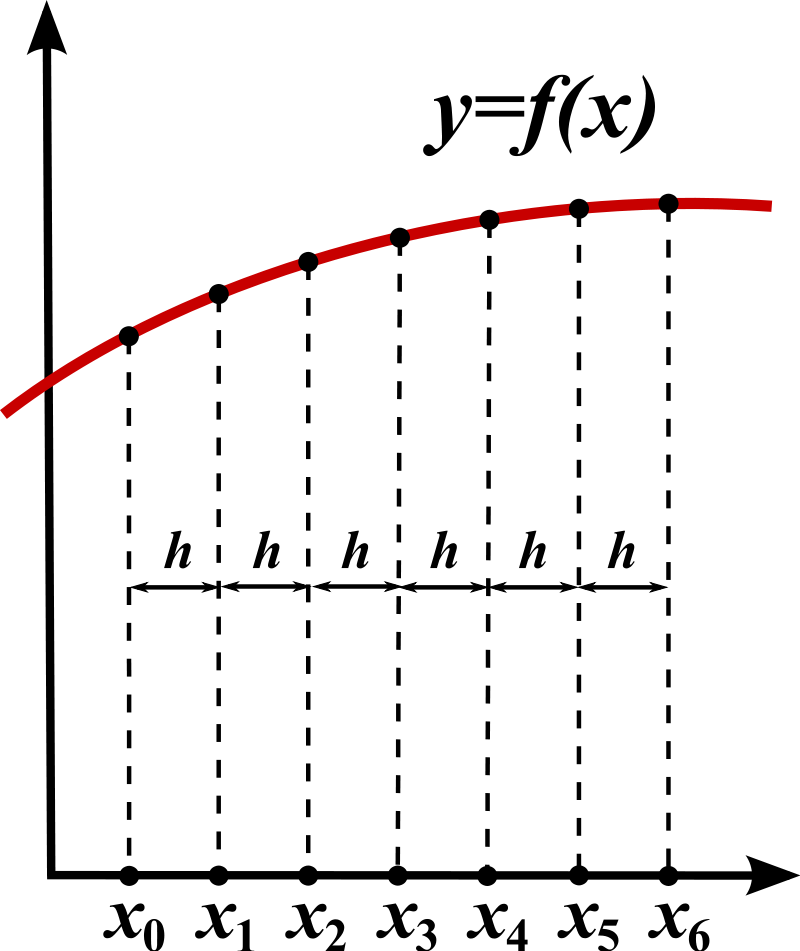
\includegraphics[width=0.5\textwidth]{graphics/800px-Finite_Differences.svg.png}
    \caption{Discretization of a continuous function y (in red) along a discrete space x ($x_0, x_1, x_2$,...).
    Every point is shifted an interval distance h.
    %Such the discrete function y of $x\in\{x_0, x_1, x_2, ...\}$ is a straight connection between the dots.
    }
    \label{fig:finite_difference}
\end{figure}
The lattice Boltzmann method is one among many to simulate the behaviour of a fluid.
Especially when it comes to numerical simulations of the thin film equation, see Eq.~(\ref{eq:simple_thin_film}), other numerical approaches are more established and have been successfully applied for more then thirty years~\cite{beckerComplexDewettingScenarios2003, peschkaSignaturesSlipDewetting2019, davidovitchSpreadingViscousFluid2005, meckeThermalFluctuationsThin2005, diezGlobalModelsMoving2000, schwartzSimulationDropletMotion1998}.
Since the thin film equation is a fourth order partial differential equation (PDE) one has to be careful in choosing an appropriate scheme.
Careful in the sense that not every numerical scheme will be able to provide first stability and second a correct approximation of the solution.
Problems for example appear when a simple Euler approach is used to solve the thin film equation.
The reason behind this complexity is the structure of the equation. 
It admits a fourth order differential in space, due to the pressure gradient, and allows for non linear behaviour.
Still though there are finite difference schemes that can be used to simulate the thin film equation.

Using finite differences means nothing more than discretizing the continuous problem into small discrete segments.
Figure~\ref{fig:finite_difference} illustrates a discretization approach where the functions is approximated by a finite set of points and intervals between them.
While it may be straightforward to attribute a value to e.g. the density $\rho(x_i) = \rho_i$ it becomes more involved for differentials.
The thin film equation admits a term which is the gradient, the pressure gradient $(\nabla p)$.
Discretization of a derivative is a long studied problem~\cite{boole1872treatise, jordan1965calculus}.
Using the Taylor expansion therefore allows to approximate a solution to the differential.
In one spatial dimension there are three different methods to compute the derivative, neglecting boundary conditions there is
\begin{equation}\label{eq:forward_dif}
    \partial_x f(x_i) = \frac{f(x_{i+1}) - f(x_i)}{h},
\end{equation}
where $h$ is the spacing between two consecutive points as introduced in Fig.~\ref{fig:finite_difference}. 
Subtracting the value of the function $f(x_{i+1})$ from $f(x)$ is called forward difference.
Changing the interval the backward difference is given as
\begin{equation}\label{eq:backward_dif}
    \partial_x f(x_i) = \frac{ f(x_i) - f(x_{i-1})}{h}.
\end{equation}
Both the forward as well as the backward differential are first order in their error, beyond first order is the central difference approach
\begin{equation}\label{eq:center_diff}
    \partial_x f(x_i) = \frac{ f(x_{i+1}) - f(x_{i-1})}{2h},
\end{equation}
where the value of the derivative is averaged over a larger interval. 

However all finite difference schemes suffer from the concrete choice of the discretization, which is often referred as discritization artifacts.
Since the starting equation is usually a continuous one in both space and time one needs to discretize the system. 
This can be done as shown in Fig.~\ref{fig:finite_difference} by introducing a lattice for the spatial dimensions. 
Time stepping is another problem but for now it is sufficient to think of time in terms of a one dimensional lattice as well. 
To understand the error one makes using finite difference think of a sine wave and mark two points along the curve.
Connecting them yields a straight line and therefore all information in between the points is lost, instead of $y(x) = \sin(x)$ one would guess $y(x) = kx + d$ for the points.
Besides the fact that information about the function is lost it still could be a good enough approximation for the derivative, especially if the points are not too far apart.
Increasing the number of points along the curve will increase the accuracy of the resulting approximation as displayed in Fig.~\ref{fig:finite_difference}.
In that sense it is necessary to sample more than two points to understand that the function is $\sin(x)$.
Which explains the so called fidelity of the finite difference method~\cite{GURUSWAMY200231}.
One needs a fine enough grid to resolve the to be studied dynamics, but the smaller the lattice spacing gets the more numerically demanding is the calculation.

\subsection{Finite differences}
In fact there are further limitations to the problem of numerically approximating a partial differential equations.
Numerical methods for partial differential equations, e.g. the thin film or the wave equation, need to satisfy the Courant Friedrichs Lewy condition (CFL)~\cite{courant1928partiellen}.  
Which beyond other things states that choosing a increment for time can not be independent of the spatial resolution.
This can be written as
\begin{equation}\label{eq:CFL}
    C = \Delta t \left(\sum_{i=1}^n \frac{u_{x_i}}{\Delta x_i}\right) \leq C_{max},
\end{equation}
with $\Delta x_i$ and $\Delta t$ being the spatial and temporal increment, respectively and $u_{x_i}$ being the magnitude of the velocity in the respective direction.
Behind this concept is the idea that propagation of information has a upper limit.
For fluid dynamic problems one speaks about the speed of sound, in electrodynamics it would be the speed of light on the other hand.
Any propagation larger than this upper limit introduces stability issues, e.g. blow ups.
Thinking about a wave package, numerically it should be ensured that several time iterations happen before the package has reached the next point of the spatial resolved lattice.
$C_{max} = 1$ for an explicit solver to which for example the lattice Boltzmann method belongs (assuming a BGK collision operator).
But can be relaxed to be larger than one for implicit methods.
In Fig.~\ref{fig:finite_difference} there is a single lattice constant $h$ that sets the spatial resolution of the system as such $\Delta x = h$.
Time stepping thus the step from $u(x_i,t_0)$ to $u(x_i,t_1)$ can ensure that forces and therefore acceleration are well within the stability condition.
Concerning the thin film equation a rather well working scheme is the Crank-Nicolson approach~\cite{crank_nicolson_1947, diezGlobalModelsMoving2000, 10.5555/1403886}.

\subsection{Spectral methods}
Of course it is as well possible to perform a transformation and solve the differential equation in Fourier space, or in other words perform a Fourier Transformation (FT), which was used to find the dispersion relation in Sec.~\ref{sec:thin_films}.
The set of solvers using a FT to solve a given differential equation is called spectral methods.
Doing so has the advantage of interchanging the derivatives with simple multiplications.
For example the term $\partial_x f(x)$ transforms to  
\begin{equation}\label{eq:fourier_transform}
    \partial_x f(x) = k\cdot \tilde{f}(k),
\end{equation}
where $\tilde{f}(k)$ is the Fourier transformed of $f(x)$, e.g. $\tilde{f}(k) = \delta(k - a/2\pi)$ for $f(x) = e^{iax}$. 
Instead of solving a differential equation one solves an algebraic equation, or a set of algebraic equations.
While it is often straightforward to perform the transformation is can become problematic to perform the backward transformation. 
Usually the expressions are fairly complicated and often the backward transformation into real space is not easy to perform.
Numerically speaking the operators for transformations are matrices, which usually depend on the explicit problem.
Solutions are generated by inversion of these operators and therefore by inversion of an (arbitrary) matrix.
Computing the inverse of a matrix is a demanding problem. 
Nevertheless these transformation approaches are often quite helpful finding an exact solution.
One rather prominent example is the computation of Green's functions, e.g. in electrostatics~\cite{eyges2012classical, green1889essay}.
For the shallow water theory, see Sec.~\ref{sec:theory_shallow_water} one class of effective methods are the discontinous Galerkin methods~\cite{ern2013theory}.
To the best of my knowledge this approach has not extensively been used on the thin film equation.

\subsection{Molecular dynamics}
Yet another approach that is the molecular dynamics method~\cite{haile1992molecular, zhangMolecularSimulationThin2019, doi:10.1063/1.1290698}.
Although when thinking of the motion molecules one does not think of the flow a \textbf{thin} film, molecular dynamics can be very insightful when dealing with thin film problems such as slip~\cite{jabbarzadeh1999wall, sega2013regularization}. 
Instead of working with macroscopic fields, such as density $\rho$ or velocity $\mathbf{u}$, the method uses a bottom up approach.
The main idea is to compute the trajectory of every particle using Newtons equation of motion, therefore assume particles are classical objects.
Interactions as well as boundary conditions can be added via potentials which act on particles.
A common interaction potential is the Lennard-Jones potential
\begin{equation}\label{eq:Len-Jon}
    U(r_{ij}) = 4\varepsilon\left[\left(\frac{\sigma}{r_{ij}}\right)^{12}-\left(\frac{\sigma}{r_{ij}}\right)^6\right],
\end{equation}
where $ij$ denotes the particle pair, $\varepsilon$ and $\sigma$ are the model dependent energy and length parameters respectively.
Clearly this approach is rather elegant.
Knowing the correct values for $\sigma$ and $\varepsilon$, the simulations show good agreement with experiments~\cite{zhangMolecularSimulationThin2019}.
However there is no free lunch. 
Because of the microscopic nature of this method it is compute intensive.
Per definition the method needs to know the position of every particle as well as its velocity.
But what really eats up all computing power is the computation of the potentials and therefore forces acting on the particles.
This surmounts to a lot of computational resources for small physical volumes, which is in the context of fluid flows and film formation problematic.
Assuming a box of a few nanometers in all directions and a physical time of about a picosecond ($10^{-12}s$) is already quite a lot to do for a common laptop.
Clearly a lot is depending on the implementation of the algorithm. 
There are well developed and supported software solutions that not only scale well but have an mature user interface, e.g. LAMMPS and GROMACS~\cite{PLIMPTON19951, BERENDSEN199543, lindahl2001gromacs}.  
However all development can not overcome that this method is suited only for relatively small systems and not for macroscopic scales.
On top comes the development of interaction potentials that due their complexity can not easily understood anymore.
Water for example although the most prominent liquid in our life is rather complex substance.
There exists not a single model for how water should interact but several, all with very fine tuned adjustments.
Without knowing why a certain water model is more suited than another one, this approach can come down to a black box.
Of course, similar to other parts of computational physics, all results need to be tested with an experiment but using molecular dynamics correct may require a lot more knowledge than e.g. finite differences.

\section{The Lattice Boltzmann Method}\label{sec:LBM}
\begin{figure}
    \centering
    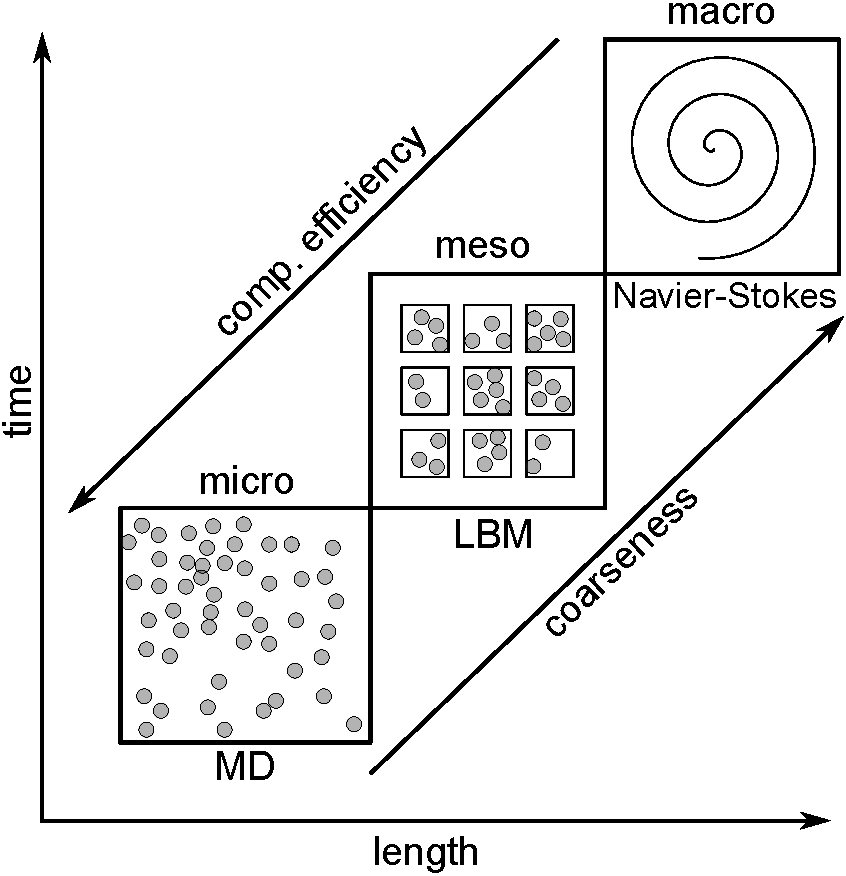
\includegraphics[width=0.95\textwidth]{graphics/Scales_problem.pdf}
    \caption{Schematic display of how different approaches relate to different length and time scales.
    The finer the system is resolved the more computing resources are needed.}
    \label{fig:scales_dummy}
\end{figure}
The lattice Boltzmann method is as the name suggests a discretization approach to the Boltzmann equation~\cite{krugerLatticeBoltzmannMethod2017, succi, wolf-gladrow}.
Boltzmann more then a hundred years ago introduced a model that was build on the assumptions that atoms and molecules move classically.
This was actually just a small portion of his groundbreaking work which forms a whole subsection of physics called statistical mechanics. 
He as well knew that there are a lot of oxygen, nitrogen and other atoms that make up the content of air we inhale with a single breath.
In 1811 already Avogadro calculated that rough number of molecules and around fifty years later Loschmidt came to a similar result~\cite{avogadro1811essai, loschmidt52grosse}
\begin{equation}
    n = \frac{p N_A}{R T},
\end{equation}
where $n$ is the number density, $p$ the pressure, $R$ the gas constant and $T$ the temperature.
The constant named after Avogadro ($N_A$) states that a mole of some substance has about $6 \cdot 10^{23}$ atoms.
Boltzmanns ingenious idea, this adjective is justified as even mathematicians find statistical mechanics appealing, to solve the dynamics of this complex coupled system was to use an statistical ansatz.
Instead of solving the equations of motion for every particle, which is the idea of molecular dynamics as introduced above, Boltzmann decided to introduce distribution functions $f(\mathbf{x},{\boldsymbol\xi},t)$, which depend on position, momentum and time and generate an ensemble.
Figure~\ref{fig:scales_dummy} illustrates the idea coming from either a macroscopic system or a microscopic system.
Instead of dealing with every atom or molecule, which is displayed in the bottom left of the figure, it is also possible to use a more coarse approach. 
Which is shown in the middle of the figure where distributions over ensembles of particles are used~\cite{raabe2004overview}.
Therefore instead of working in the microscopic world the lattice Boltzmann method works in a mesoscopic regime.
Making it computationally more efficient for larger class of problems.
Of course, it is also possible to use a coarser approach and in fact a lot of the classical Navier-Stokes solvers operate in the upper right of Fig.~\ref{fig:scales_dummy}, see Chap.~\ref{chapter:fourth_paper} for some example solvers.

\subsection{The Boltzmann equation}
The dynamics of this distributions $f$ can be formalized and put into an evolution equation which is called the Boltzmann equation
\begin{equation}\label{eq:boltzmann_eq}
    \partial_t f + {\boldsymbol\xi}\cdot\nabla f + \frac{1}{\rho}\mathbf{F}\cdot\partial_{{\boldsymbol\xi}}f = \Omega(f), 
\end{equation}
where ${\boldsymbol\xi}$ is the momentum and the first two terms describe the advection of the distribution due to the atoms and the third term measures the effect of a force $\mathbf{F}$ on the momentum~\cite{krugerLatticeBoltzmannMethod2017}.
On the right side of the equation is an arbitrary complex term, the collision operator.
This operator accounts for all collisions the atoms or particles perform at any given instance of time.
In principle this operator can not be computed analytically, because one need to integrate out the whole phase space $(\int \diff^3\mathbf{x}, \int \diff^3\xi)$ for all possible collision terms, therefore for the two up to n-point interactions. 

However with a smart ansatz it is possible to find a suitable approximation to the collision operator.
The easiest ansatz one can make is
\begin{enumerate}
    \item The fluids state is not far of its equilibrium.
    \item During the collision it approaches its equilibrium with a relaxation time $\tau$.
\end{enumerate}
Bhatnagar, Gross and Krook (BGK) were the first ones who worked out the mathematical model behind this ansatz~\cite{PhysRev.94.511}.
This model can be formalized quite simply and reads
\begin{equation}
    \Omega(f) = -\frac{1}{\tau}(f - f^{eq}),
\end{equation}
where $f^{eq}$ denotes the equilibrium distribution function.
The moments of the BGK collision operator satisfy the following set of equations
\begin{align}
    \int \Omega(f) \diff^3\xi = 0, \label{eq:BGK_1}\\
    \int {\boldsymbol\xi}\Omega(f) \diff^3\xi = \mathbf{0}, \label{eq:BGK_2}\\
    \int |{\boldsymbol\xi}|^2\Omega(f) \diff^3\xi = 0, \label{eq:BGK_3}\\
    \int |\mathbf{v}|^2\Omega(f) \diff^3\xi = 0. \label{eq:BGK_4}
\end{align}
The first of the above equations states that the mass is conserved, while Eq.~(\ref{eq:BGK_2}) ensures momentum conservation.
Eqs.~(\ref{eq:BGK_3}, \ref{eq:BGK_4}) tell us that both that the total energy as well as the internal energy are conserved.
Taking this four constraints into consideration as well as the points 1. and 2. one finds that the BGK operator is the simplest one to satisfy them all.
With one side note however, the full collision operator from Boltzmann does predict a different Prandtl number ($Pr$) than the BGK yields.
The Prandtl number $Pr = \nu/\alpha$ measures viscosity against thermal diffusivity ($\alpha$). 
Using BGK one gets $Pr=1$ while monoatomic gases or Boltzmann's operator showing $Pr\simeq 2/3$~\cite{cercignani1988boltzmann, krugerLatticeBoltzmannMethod2017}.

\subsection{Lattice Boltzmann and Chapman Enskog}
Since the method got first developed in the 1986 it has gained more and more popularity~\cite{PhysRevLett.56.1505}.
Due the simplicity of the method a lot has been worked out over last fourty years.
The reason why the lattice Boltzmann method is lacking behind when it comes to thin films flows is due to it's origin as an approximation to the Navier-Stokes equation.
That said there are of course studies of thin film flows using the lattice Boltzmann method, e.g. Sbragaglia et al.~\cite{Sbragaglia}.
However they rely on additional contributions for either multiphase or multicomponent models~\cite{shan1993lattice, shan_yuan_chen_2006, CHEN1995617}.
To actually solve Eq.~(\ref{eq:boltzmann_eq}) a few steps are still missing.
First being the discretization of the equation.
Now as the name suggests a lattice with lattice constants $\Delta x$ and $\Delta t$ for spatial and temporal discretization is the desired domain.
A first guess of this discretization on Eq.~(\ref{eq:boltzmann_eq}) could be
\begin{equation}\label{eq:LBM_discret_noforces}
    f_{\alpha}(\mathbf{x}+\mathbf{c}_{\alpha}\Delta t, t+ \Delta t) - f_{\alpha}(\mathbf{x}, t) = -\frac{\Delta t}{\tau}(f_{\alpha}(\mathbf{x}, t) - f^{eq}_{\alpha}(\mathbf{x}, t)),
\end{equation}
where the $\mathbf{c}_{\alpha}$ form a discrete set of $\alpha$ velocities.
Although this guess may seem different (\textit{simpler}) than Eq.~(\ref{eq:boltzmann_eq}) Chapman and Enskog have shown that this does not only resembles the Boltzmann equation but also is an approximation to the Navier-Stokes equation~\cite{chapmanMathematicalTheoryNonuniform1990, enskogKinetischeTheorieVorgange1917}. 
The idea is to derive a perturbation expansion of the distribution functions around their equilibrium as such
\begin{equation}\label{eq:expansion_f}
    f_{\alpha} = f_{\alpha}^{eq} + \epsilon f_{\alpha}^{(1)} + \epsilon^2 f_{\alpha}^{(2)} + O(\epsilon^3), 
\end{equation}
where $\epsilon$ accounts for the order in Knudsen number ($Kn$). 
$Kn = \lambda/L$ is a measure to compare the mean free path to a characteristic length scale, i.e. ballistic and diffusive regime.
Introducing the non-equilibrium part of the distribution $f$ as $f^{neq} = f - f^{eq}$. 
They as well have to satisfy 
\begin{align}\label{eq:non_constraint}
    \sum_{\alpha} f_{\alpha}^{neq} = 0, \\
    \sum_{\alpha} \mathbf{c}_{\alpha}f_{\alpha}^{neq} = 0, 
\end{align}
where due to discretization the integration of Eqs.(\ref{eq:BGK_1}-\ref{eq:BGK_4}) becomes a sum.
The moments of the equilibrium functions on the other hand need to satisfy~\cite{chen1998lattice} 
\begin{align}
    \Pi^{eq} &= \sum_{\alpha} f_{\alpha}^{eq} = \rho, \label{eq:moments_equilibria_1}\\
    \Pi^{eq}_i &= \sum_{\alpha} c_{\alpha i}f_{\alpha}^{eq} = \rho u_i, \label{eq:moments_equilibria_2}\\
    \Pi^{eq}_{i j} &= \sum_{\alpha} c_{\alpha i} c_{\alpha j}f_{\alpha}^{eq} = \rho u_i u_j + \rho c_s^2\delta_{i j}, \label{eq:moments_equilibria_3}\\
    \Pi^{eq}_i &= \sum_{\alpha} c_{\alpha i} c_{\alpha j} c_{\alpha k}f_{\alpha}^{eq} = \rho c_s^2(u_i\delta_{j k} + u_j\delta_{k i} + u_k\delta_{i j}), \label{eq:moments_equilibria_4}
\end{align}
In fact for every order of expansion Eq.~(\ref{eq:expansion_f}) one gets
\begin{align}\label{eq:all_order_constraint}
    \sum_{\alpha} f_{\alpha}^{(n)} = 0, \\
    \sum_{\alpha} \mathbf{c}_{\alpha}f_{\alpha}^{(n)} = 0. 
\end{align}

Performing a Taylor expansion of Eq.~(\ref{eq:boltzmann_eq}) with a discrete set of velocities assuming no force is present yields~\cite{krugerLatticeBoltzmannMethod2017}
\begin{equation}\label{eq:Taylor_discret_boltzmann}
    \Delta t (\partial_t + c_{\alpha i}\partial_i)f_{\alpha} + \frac{\Delta t^2}{2}(\partial_t + c_{\alpha i}\partial_i)^2 f_{\alpha} + O(\Delta t^3) = -\frac{\Delta t}{\tau} f_{\alpha}^{neq}.
\end{equation}
Leaving higher orders aside one finds that this is actually a slow mode expansion of $f_{\alpha}$.
Meaning that $f_{\alpha}$ changes only with macroscopic time scales, if this is not ensured higher orders needs to be considered.
Subtracting $\Delta t/2 (\partial_t + c_{\alpha i}\partial_i)$ from both sides yields
\begin{equation}\label{eq:derive_lbm_orders}
    \Delta t (\partial_t + c_{\alpha i}\partial_i)f_{\alpha} = -\frac{\Delta t}{\tau} f_{\alpha}^{neq} + \Delta t (\partial_t + c_{\alpha i}\partial_i)\frac{\Delta t}{2\tau} f^{neq}_{\alpha},
\end{equation}
which is first order in derivatives.
The time and especially the time derivatives need also to be expanded in orders of $Kn$ and therefore
\begin{equation}\label{eq:expansion_time}
    \Delta t \partial_t f_{\alpha} = \Delta t (\epsilon\partial_t^{(1)} + \epsilon^2\partial_t^{(2)} + O(\epsilon^3)) f_{\alpha}.
\end{equation}
For the spatial deviates it is sufficient to use
\begin{equation}\label{eq:expansion_space}
    \Delta t c_{\alpha i}\partial_i f_{\alpha} = \Delta t(\epsilon c_{\alpha i}\partial_i^{(1)}) f_{\alpha}.
\end{equation}
With a note of caution for Eq.~(\ref{eq:expansion_time}) as only the sum of all orders in $\epsilon$ resembles the real time derivative.
Applying both expansions Eq.~(\ref{eq:expansion_f}) and Eq.~(\ref{eq:expansion_time}) to Eq.~(\ref{eq:derive_lbm_orders}) we have
\begin{equation}\label{eq:first_order_esp}
    (\partial_t^{1} + c_{\alpha i}\partial_{i}) f_{\alpha}^{eq} = -\frac{\Delta t}{\tau} f_{\alpha}^{(1)}
\end{equation}
at first order in $\epsilon$ and 
\begin{equation}\label{eq:sec_order_esp}
    \partial_t^{2} f_{\alpha}^{eq} + (\partial_t^{1} + c_{\alpha i}\partial_{i})\left(1 - \frac{\Delta t}{2\tau}\right) f_{\alpha}^{(1)} = -\frac{\Delta t}{\tau} f_{\alpha}^{(2)},
\end{equation}
for $O(\epsilon^2)$.

Taking the moments of Eq.~(\ref{eq:first_order_esp}), see Eqs.(\ref{eq:moments_equilibria_1}-\ref{eq:moments_equilibria_4}) yields
\begin{align}
    \partial_t^{(1)}\rho + \partial_j^{(1)}(\rho u_j) &= 0, \label{eq:cont_lbm}\\
    \partial_t^{(1)}(\rho u_i) + \partial_j^{(1)}\Pi^{eq}_{ij} &= 0, \label{eq:mom_lbm}\\
    \partial_t^{(1)}\Pi^{eq}_{ij} + \partial_k^{(1)}\Pi^{eq}_{ijk} &= -\frac{1}{\tau}\Pi^{(1)}_{ij}, \label{eq:energy_lbm}
\end{align}
for which the moments $\Pi$ are
\begin{align}
    \Pi^{eq}_{ij} &= \sum_{\alpha}c_{\alpha i} c_{\alpha j} f_{\alpha}^{eq} = \rho u_i u_j + \rho c_s^2\delta_{i j}, \label{eq:Pi_lbm_1}\\
    \Pi^{eq}_{ijk} &= \sum_{\alpha}c_{\alpha i} c_{\alpha j} c_{\alpha k} f_{\alpha}^{eq} = \rho c_s^2(u_i\delta_{j k} + u_j\delta_{k i} + u_k\delta_{i j}), \label{eq:Pi_lbm_2}\\
    \Pi^{(1)}_{ij} &= \sum_{\alpha}c_{\alpha i} c_{\alpha j} f_{\alpha}^{(1)}, \label{eq:Pi_lbm_3}
\end{align}
where Eqs.~(\ref{eq:moments_equilibria_1}-\ref{eq:moments_equilibria_4}) have been used.
Interestingly Eq.~(\ref{eq:cont_lbm}) and Eq.~(\ref{eq:mom_lbm}) resemble the continuity and Euler momentum equation, this is not by chance.

Taking the moments of Eq.~(\ref{eq:sec_order_esp}) we have
\begin{align}
    \partial_t^{(2)}\rho &= 0, \\
    \partial_t^{(2)}(\rho u_i) + \partial^{(1)}_j\left(1 - \frac{\Delta t}{2\tau}\right)\Pi_{i j}^{(1)} &= 0.
\end{align}
As there is now an equation for $\Pi^{(1)}_{i j}$ it is possible to collect the mass and momentum equation for both $O(\epsilon)$ and $O(\epsilon^2)$
\begin{align}
    (\epsilon\partial_t^{(1)} + \epsilon^2\partial^{(2)})\rho + \epsilon\partial_i^{(1)}(\rho u_i) &= 0, \\
    (\epsilon\partial_t^{(1)} + \epsilon^2\partial^{(2)})(\rho u_i) + \epsilon\partial_j^{(1)}\Pi^{eq}_{i j} &= -\epsilon^2\partial_j^{(2)}\left(1 - \frac{\Delta t}{2\tau}\right) \Pi^{(1)}_{i j}. 
\end{align}
This system in fact resembles the Navier-Stokes with the small pitfall that the viscous stress tensor
\begin{equation}
    \sigma = - \left(1 - \frac{\Delta t}{2\tau}\right) \Pi^{(1)},
\end{equation}
is as of now still unknown.
Cut the last part short for an isothermal equation of state and $f^{eq}$ as function of $O(u^2)$ for example
\begin{equation}\label{eq:eqi_dist1}
    f_{\alpha}^{eq} = \rho(a + b c_{\alpha i} u_i + d (c_{\alpha i} u_i)^2 + e u^2),
\end{equation}
then the tensor is given as
\begin{equation}
    \Pi^{(1)} = -\rho c_s^2\tau(\partial_j^{(1)}u_i + \partial_i^{(1)}u_j) + \tau\partial_k^{(1)}(\rho u_i u_j u_k),
\end{equation}
which concludes the expansion part.
So far however no assumptions on the lattice distributions are made and the equilibrium distribution function has not been specified.
Paving work by He and Luo as well as group theoretical arguments derived by Rubinstein and Luo showed that based on dimensionallity just a few (discrete) velocities are sufficient~\cite{heTheoryLatticeBoltzmann1997, rubinstein2008theory}.
In fact in Chap.~\ref{chapter:first_paper} all numerical experiments were performed on a D2Q9 lattice therefore $\mathbf{c}_{\alpha}$ is
\begin{equation}\label{eq:speeds_method}
\mathbf{c}_{\alpha}  =
\left\{
\begin{array}{ll}
(0,0) & \alpha = 0 \\
\left[\cos{\frac{(\alpha-1)\pi}{4}}, \sin{\frac{(\alpha-1)\pi}{4}} \right] &  \alpha=1,3,5,7 \\
\sqrt{2}\left[\cos{\frac{(\alpha-1)\pi}{4}}, \sin{\frac{(\alpha-1)\pi}{4}} \right] & \alpha=2,4,6,8
\end{array}
\right.,
\end{equation}
The only missing pieces are $a, b, c, d$ of Eq.~(\ref{eq:eqi_dist1}).
Using the set of equations~(\ref{eq:moments_equilibria_1}-\ref{eq:moments_equilibria_4}) one quickly finds
\begin{equation}
    a = 1,\quad b = \frac{1}{c_s^2},\quad d = \frac{1}{2c_s^4},\quad e = \frac{1}{2c_s^2},
\end{equation}
however with the addition of lattice weights to ensure the H-theorem~\cite{krugerLatticeBoltzmannMethod2017}
\begin{equation}\label{eq:weightsD2Q9_meth}
w_{\alpha} = \begin{cases}
4/9 &\text{$\alpha = 0$}\\
1/9 &\text{$\alpha = 1,2,3,4$}\\
1/36 &\text{$\alpha = 5,6,7,8$}
\end{cases}
,
\end{equation}
such that the equilibria can be written as
\begin{equation}\label{eq:eqi_dist2}
    f_{\alpha}^{eq} = w_{\alpha}\rho\left(1 + \frac{c_{\alpha i} u_i}{c_s^2} +  \frac{(c_{\alpha i} u_i)^2}{2c_s^4} + \frac{u^2}{2c_s}\right).
\end{equation}
Together with the evolution equation Eq.~(\ref{eq:LBM_discret_noforces}) it is therefore possible to approximate the Navier-Stokes, at least in regimes of small Knudsen and Mach numbers, $Kn = Ma \ll 1$.

The idea however of this thesis is not to approximate the Navier-Stokes equation but have a numerical solver for the thin film equation.
Luckily for me and as outlined in Chap.~\ref{chapter:theory} there is a system which has some similarities with the thin film equation.
That system is the shallow water equation. 
In fact it is possible to derive with an similar ansatz, e.g. a slow mode expansion, the shallow water equation from the Boltzmann equation~\cite{salmonLatticeBoltzmannMethod1999, zhouLatticeBoltzmannMethods2004, dellarNonhydrodynamicModesPriori2002}.
While Eq.~(\ref{eq:LBM_discret_noforces}) does not need to be modified the shallow water equations require a different equilibrium distribution.
Instead of an isothermal equation of state $p = \rho c_s^2$, the shallow water system uses the hydrostatic pressure Eq.~(\ref{eq:hydro_static_int}) as closure.

In Chap.~\ref{chapter:first_paper} the modified equilibrium distribution function will be presented and motivated. 
They will be the starting point to find constructive matching conditions between the shallow water model and the thin film equation.
Meaning not only does the equilibrium have to be changed but to account for thin film dynamics such as wetting, see Eq.~(\ref{eq:disjoin_p}), forces will be introduced.
Most importantly to mention is the friction with the substrate as such the no-slip or Navier-slip condition and the disjoining pressure.

The derivation of the lattice Boltzmann method and outline of the modified approach for thin film flows concludes this chapter now.
Following is a chapter about the sustainable approach I choose to keep the software first of all Open Source and maintainable for years to come.
After the introduction of \textit{Swalbe.jl} in Chap.~\ref{chapter:fourth_paper} the method is thoroughly tested against problems such as the Rayleigh-Taylor instability in Chap.~\ref{chapter:first_paper}.
While in Chap.~\ref{chapter:second_paper} an additional contribution due to thermal fluctuations is considered. 
Although the focus is solemnly on thermal fluctuations, this chapter should server a guideline for the inclusion of further dynamics.
